\documentclass[a4paper,12pt]{report}
\usepackage[utf8]{inputenc}
\usepackage[T1]{fontenc}
\usepackage[french]{babel}
\usepackage{geometry}
\usepackage{graphicx}
\usepackage{float}
\usepackage{longtable}
\usepackage{hyperref}
\usepackage{listings}
\usepackage{tikz}
\usepackage[pages=some]{background}


%--------------------------------------------------------
% Couleurs de la charte ENSTA
%--------------------------------------------------------
\definecolor{bleuENSTA}{HTML}{002A4B}
\definecolor{corailENSTA}{HTML}{F05A28}
\definecolor{grisENSTA}{gray}{0.3}



\geometry{margin=2.5cm}
\lstset{
    basicstyle=\ttfamily\small,
    frame=single,
    language=Python,
    breaklines=true,
    showstringspaces=false
}

\title{Rapport de Projet \\ \textbf{Les Aventuriers du Rail}}
\author{Zachary BARBON-EVIS \\ Lancelot RAMIS}
\date{10/05/2025}


\begin{document}
\backgroundsetup{
  scale=1,
  angle=0,
  opacity=0.5,
  contents={
    \begin{tikzpicture}[remember picture, overlay]
      \shade[inner color=bleuENSTA!60, outer color=white]
        (current page.north west) circle (20cm);
      \shade[inner color=bleuENSTA!60, outer color=white]
        (current page.south east) circle (25cm);
    \end{tikzpicture}
  }
}
\BgThispage

\maketitle
\tableofcontents

\chapter*{Introduction}
\addcontentsline{toc}{chapter}{Introduction}

\textit{Les Aventuriers du Rail} est un jeu de société stratégique dans lequel les joueurs collectent des cartes pour
construire des lignes de chemin de fer entre des villes d’un continent. Chaque joueur tente de remplir des objectifs
secrets tout en bloquant, si possible, les adversaires. Le jeu repose sur la prise de décisions tactiques,
la gestion de ressources, et une vision globale du plateau.

Dans le cadre de notre formation en informatique, ce projet a pour but de traduire ces mécaniques ludiques en une
architecture logicielle modulaire et cohérente. Il constitue une application concrète de la programmation orientée objet,
de la modélisation par diagrammes de classes, et de la structuration de projet.
Il s’inscrit également dans une démarche progressive, où l’on passe d’un modèle de jeu manuel à une simulation
automatique puis intelligente, tout en respectant des contraintes de clarté, de testabilité et d’extensibilité du code.

Le projet repose sur plusieurs objectifs pédagogiques :
\begin{itemize}
    \item Mettre en place une modélisation complète du jeu : carte, routes, joueurs, cartes wagon et cartes objectif.
    \item Déterminer et implémenter les actions possibles à chaque tour, en respectant les règles du jeu.
    \item Proposer un joueur automatique, d’abord aléatoire, puis optimisé pour chercher à atteindre ses objectifs.
    \item Calculer les scores en prenant en compte les objectifs réalisés, les routes posées et le plus long chemin.
    \item (Optionnel) Améliorer l'expérience utilisateur avec une aide au jeu, une IHM graphique ou des alertes intelligentes.
\end{itemize}

Ce rapport présente l’état actuel de l’avancement, la structure générale du programme, les principales classes et méthodes,
ainsi que les perspectives pour la suite du développement.

\chapter{Analyse du problème}

\section{Définition exacte du problème}

Le projet consiste à modéliser informatiquement une version simplifiée du jeu de société \textit{Les Aventuriers du Rail}.
Il s'agit de simuler le déroulement d'une partie à l'aide d'une modélisation orientée objet, en respectant les règles de base du jeu original.

Le cœur du problème réside dans la mise en place d'une structure de données représentant :
\begin{itemize}
    \item la carte du jeu (un graphe dont les sommets sont des villes et les arêtes sont les routes disponibles) ;
    \item les joueurs, chacun possédant un stock de wagons, des cartes wagon, et des objectifs à remplir ;
    \item les actions possibles à chaque tour : piocher des cartes wagon, capturer une route, ou éventuellement choisir
    de nouveaux objectif (option désactivée pour le joueur automatique dans notre simplification) ;
    \item les règles du jeu, notamment les contraintes de pioche, la capture de routes grises
    (par n'importe quelle couleur), et la limitation à deux actions maximum par tour ;
    \item la mise à jour du plateau à chaque action, avec vérification de la fin de partie.
\end{itemize}

Le système doit également permettre d’attribuer les cartes d’objectifs et de wagon en début de partie,
de déterminer les coups possibles à chaque tour et de les exécuter, tout en assurant le suivi du score.

En plus de cette modélisation du jeu pour un joueur humain, le projet intègre une logique de joueur automatique
(aléatoire ou intelligent) permettant de tester plus rapidement les mécaniques.
Enfin, le calcul des scores repose sur des structures de graphe : composantes connexes pour la vérification des objectifs,
et algorithme de parcours pour identifier le plus long chemin.

Ce projet a donc pour but de fournir une simulation fidèle, évolutive et testable du jeu, en mettant l'accent sur
une organisation modulaire et une structuration orientée objet claire.

\section{Domaines d’utilisation}

Le programme développé a vocation à être utilisé dans plusieurs contextes pédagogiques ou expérimentaux.

\begin{itemize}
    \item \textbf{Aide au joueur humain} : en simulant la partie, le programme peut rappeler les objectifs en cours,
    les routes encore disponibles, ou avertir lorsqu’un objectif devient difficile voir impossible à atteindre.
    Des fonctionnalités supplémentaires pourront également conseiller des actions possibles à un joueur réel.

    \item \textbf{Test de stratégie} : en comparant les performances de joueurs automatisés avec des comportements
    différents (aléatoire, optimisé, prudent, etc.), le programme permet d’analyser l'efficacité de différentes
    stratégies sur un même plateau.

    \item \textbf{Expérimentation d’un joueur automatique} : une première version aléatoire du joueur permet de tester
    les règles du jeu. À terme, l’intégration d’un joueur intelligent ouvre la voie à des travaux sur l’optimisation,
    la recherche de chemins, et l’intelligence artificielle rudimentaire.

    \item \textbf{Application pédagogique} : le projet illustre de nombreux concepts de l’enseignement en informatique :
    modélisation par classes, graphe orienté, algorithmes de parcours, règles de gestion, tests unitaires,
    documentation, et structuration en modules.
\end{itemize}

\section{Limites et simplifications}

Afin de rendre le projet plus accessible et réalisable dans un cadre pédagogique limité,
plusieurs simplifications ont été mises en place :

\begin{itemize}
    \item \textbf{Pas de sélection des objectifs} : chaque joueur reçoit trois cartes itinéraire qu’il est contraint de
    garder. L’action de tirer de nouveaux objectifs en cours de partie a été retirée pour les joueurs automatiques.

    \item \textbf{Trois joueurs fixes} : le nombre de joueurs est limité à trois pour éviter la complexité du
    multijoueur complet tout en conservant la richesse d’interaction entre joueurs.

    \item \textbf{Pas de routes doubles} : lorsqu’une route propose deux couleurs dans la version réelle du jeu, seule
    l’une est disponible. Cela évite de devoir gérer les graphes complexe. (pour la création du plateau de jeu, le graph
    comporte pour le moment 2 fleches)

    \item \textbf{Pas d’interface graphique complète} : une visualisation simple du graphe du plateau est proposée via
    \texttt{matplotlib}, mais aucune interface interactive n’est encore amorcée.

    \item \textbf{Aucune sauvegarde de partie} : le programme ne propose ni chargement, ni sauvegarde.
    Chaque exécution correspond à une partie unique. Cependant cette option reste envisageable et envisagée.

    \item \textbf{Calcul des scores partiellement implémenté} : les scores liés aux routes capturées sont pris en compte.
    Le calcul des points liés aux objectifs ou au plus long chemin est encore en développement.
\end{itemize}

Ces choix permettent de concentrer l’effort sur la mécanique de base du jeu, tout en préparant le terrain pour une
extension ultérieure pour la fin du projet.

\chapter{Description du programme}

\section{Organisation générale}

Le déroulement d'une partie suit les grandes étapes classiques du jeu \textit{Les Aventuriers du Rail},
adaptées ici dans une version simplifiée et pilotée par un contrôleur central (la classe \texttt{Table}).

\subsection*{Mise en place}

Au lancement du programme :
\begin{itemize}
    \item Le plateau de jeu est initialisé (chargement des villes et routes à partir d'une structure pré-définie en début de programme).
    \item Trois joueurs sont créés et reçoivent chacun un nombre initial de wagons (45), trois cartes objectif, et quatre cartes wagon.
    \item Les cartes wagon visibles sont tirées et affichées (cinq cartes).
\end{itemize}

\subsection*{Déroulement d’un tour de jeu}

Chaque tour, le joueur actif a le choix entre deux actions principales :
\begin{itemize}
    \item \textbf{Piocher des cartes wagon} :
        \begin{itemize}
            \item Il peut piocher deux cartes, visibles ou cachées.
            \item Si la première carte est une locomotive visible, le tour se termine immédiatement.
            \item Si la deuxième carte sélectionnée est une locomotive visible, les règles interdisant ce choix,
            un nouveau choix lui est demandé.
        \end{itemize}
    \item \textbf{Capturer une route} :
        \begin{itemize}
            \item Il sélectionne une route disponible.
            \item Il doit disposer du bon nombre de cartes wagon de la couleur correspondante (ou Locomotives/jokers).
            \item S’il possède les cartes requises et assez de wagons, il prend la route,
            sinon on lui demande de refaire un autre choix.
            \item Son score est mis à jour en fonction de la longueur de la route.
        \end{itemize}
    \item \textbf{Piocher une carte objectif} (non accessible au joueur auto):
        \begin{itemize}
            \item Il pioche 3 cartes de la pioche correspondante.
            \item Il choisit de garder une à 3 cartes et repose les autres le cas échéant.
        \end{itemize}
\end{itemize}

Après son action, le tour passe au joueur suivant. La partie continue ainsi jusqu'à ce qu'un joueur ait deux wagons
ou moins, déclenchant le dernier tour.

\subsection*{Schéma général du fonctionnement}

Un schéma synthétique peut représenter cette logique :

\begin{figure}[H]
    \centering
    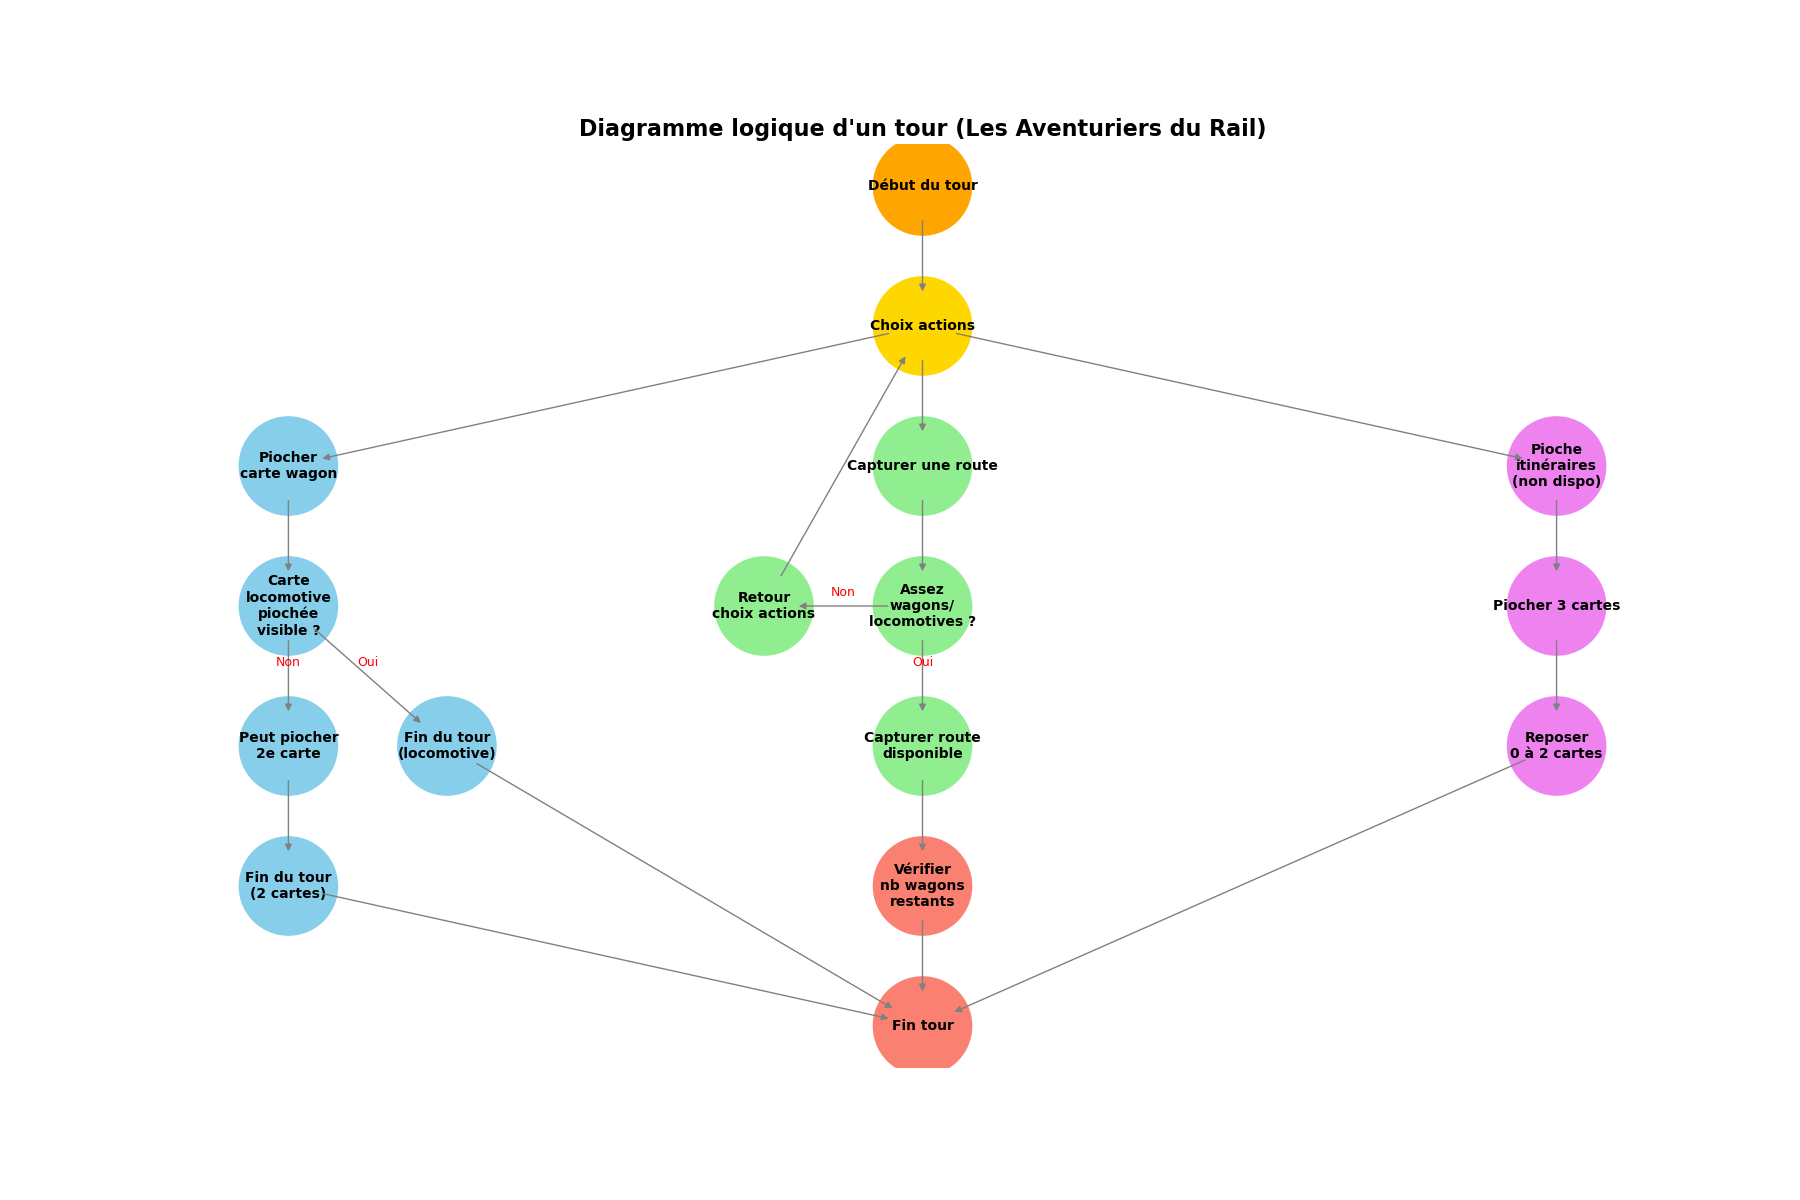
\includegraphics[width=0.9\textwidth]{graph_logique}
    \caption{Schéma du déroulement d’un tour de jeu}
    \label{fig:tour_de_jeu}
\end{figure}

\noindent Ce schéma illustre les choix possibles à chaque tour et les principales conditions vérifiées avant de poursuivre.



\section{Diagramme de classes}

\begin{figure}[H]
    \centering
    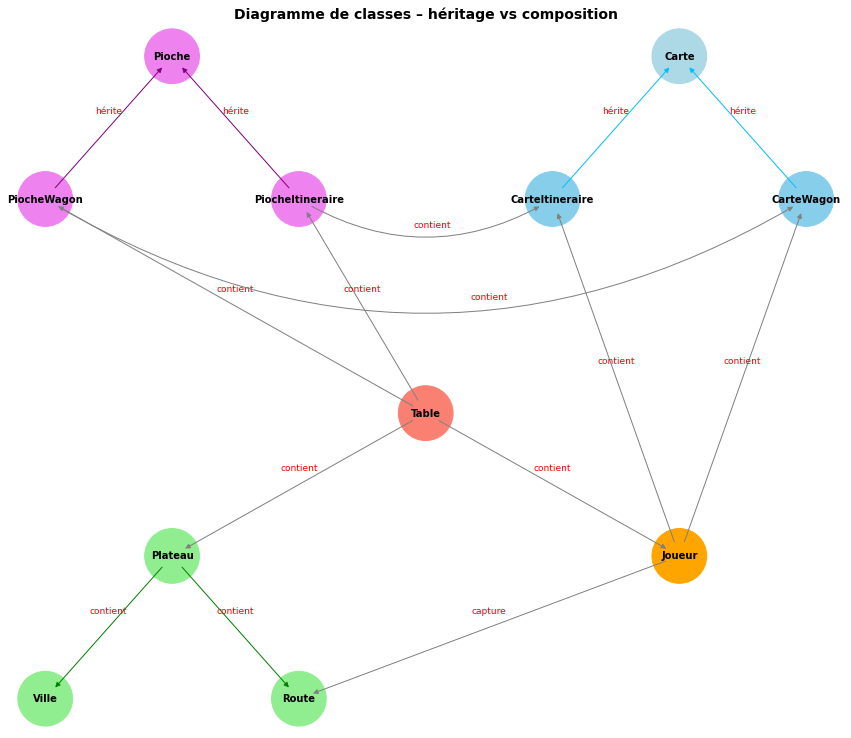
\includegraphics[width=0.9\textwidth]{diagramme_classe}
    \caption{Diagramme de classe}
    \label{fig:diagramme_classe}
\end{figure}


\section{Classes principales}

Le projet repose sur une modélisation orientée objet fidèle à la structure du jeu Les Aventuriers du Rail.
Les principales classes implémentées sont les suivantes :

\subsection*{Classe \texttt{Table}}

Cette classe coordonne la partie. Elle contient l’ensemble des objets nécessaires au déroulement du jeu :
les joueurs, le plateau, les pioches (cartes wagon et cartes itinéraire), ainsi que la gestion des tours.
C’est le point d’entrée principal de l’exécution du jeu.

\begin{itemize}
    \item Initialise les composants de la partie (joueurs, pioches, plateau, objectifs).
    \item Gère le déroulement du jeu tour par tour.
    \item Implémente les règles de pioche, de capture de route, et les contrôles de validité.
\end{itemize}

\subsection*{Classe \texttt{Joueur}}

Un joueur est caractérisé par :
\begin{itemize}
    \item Un nom, un nombre de wagons disponibles.
    \item Une main de cartes wagon et une main de cartes objectif.
    \item Un score évolutif.
\end{itemize}
Le joueur interagit avec la table en piochant, en capturant des routes, et en remplissant ses objectifs.
Des méthodes de jeu automatique seront ajoutées par la suite.

\subsection*{Classe \texttt{Plateau}}

Cette classe représente la carte du jeu, sous forme d’un graphe via \texttt{networkx}. Elle contient :
\begin{itemize}
    \item La liste des villes (sommets du graphe).
    \item La liste des routes entre villes (arêtes, avec couleur et longueur).
    \item Une méthode d'affichage graphique du plateau à l’aide de \texttt{matplotlib}.
\end{itemize}
Elle est utilisée pour déterminer les routes disponibles et afficher l’état du jeu.

\subsection*{Classes \texttt{Carte}, \texttt{CarteWagon}, \texttt{CarteItineraire}}

La classe \texttt{Carte} est une classe abstraite commune aux cartes du jeu, utilisée comme base pour organiser les
classes \texttt{CarteWagon} et \texttt{CarteItineraire}. Elle permet de regrouper certains comportements communs et de
faciliter la représentation du jeu.

\begin{itemize}
    \item \texttt{CarteWagon} hérite de \texttt{Carte} et représente une carte de couleur (ou locomotive).
    Elle contient une information sur la couleur, utilisée pour valider la capture d'une route.
    \item \texttt{CarteItineraire} hérite aussi de \texttt{Carte} et représente une carte objectif :
    elle contient deux villes et une valeur en points. L’objectif est réussi si les deux villes sont
    connectées à la fin de la partie.
\end{itemize}

\vspace{0.5em}

\subsection*{Classes \texttt{Pioche}, \texttt{PiocheWagon}, \texttt{PiocheItineraire}}

La classe \texttt{Pioche} est une classe générique pour toute pile de cartes tirables.
Elle gère l'instanciation des cartes et leur mélange.
Deux sous-classes spécialisent ce comportement :

\begin{itemize}
    \item \texttt{PiocheWagon} contient les cartes wagon, gère une pioche visible (5 cartes affichées),
    et applique les règles spécifiques du jeu (ex : une locomotive visible en premier interdit un deuxième tirage).
    \item \texttt{PiocheItineraire} contient les cartes objectif.
    Lors d’une pioche, le joueur reçoit trois cartes et doit en conserver au moins une (hors initialisation).
\end{itemize}

La séparation de ces classes facilite la gestion de règles différentes pour chaque type de carte tout en mutualisant
la logique commune dans la classe parente \texttt{Pioche}.

\subsection*{Classe \texttt{Ville}}

Une ville est un nœud du graphe du plateau généralement définie par son nom et ses coordonnées graphiques.
Elle est utilisée pour placer les routes sur le graphe et pour calculer les connexions.

\subsection*{Classe \texttt{Route}}

Une route est une liaison entre deux villes. Elle est caractérisée par :
\begin{itemize}
    \item Sa longueur (nombre de wagons nécessaires).
    \item Sa couleur (ou gris pour n’importe quelle couleur).
    \item Le joueur qui l’a capturée (ou \texttt{None} si encore disponible).
\end{itemize}
Elle est représentée par une arête dans le graphe du plateau.


\section{Méthodes importantes}

Certaines méthodes du projet jouent un rôle central dans le déroulement du jeu.
Nous présentons ici celles qui participent directement à l'exécution des actions du joueur et à la mise à jour du plateau.

\subsection*{\texttt{jouer\_tour(joueur)} — classe \texttt{Table}}

Cette méthode coordonne un tour de jeu pour le joueur donné.
Elle appelle selon les cas les fonctions de pioche ou de capture de route, puis actualise le plateau.
Elle gère les règles suivantes :
\begin{itemize}
    \item Choix entre piocher ou capturer une route.
    \item Interdiction de piocher une locomotive en deuxième carte.
    \item Passage au joueur suivant.
\end{itemize}

\subsection*{\texttt{piocher\_cartes\_wagon(joueur)} — classe \texttt{Table}}

Permet au joueur de piocher une ou deux cartes wagon. Elle intègre les règles du jeu :
\begin{itemize}
    \item Le joueur peut choisir parmi les cartes visibles ou tirer à l’aveugle.
    \item Si la première carte est une locomotive visible, le joueur ne peut pas piocher une deuxième carte.
    \item Si le joueur choisit une locomotive en deuxième carte, il est contraint de refaire un choix.
\end{itemize}

\subsection*{\texttt{capturer\_route(joueur)} — classe \texttt{Table}}

Cette méthode permet à un joueur de capturer une route, c’est-à-dire :
\begin{itemize}
    \item Vérifier qu’il possède les cartes nécessaires.
    \item Vérifier qu’il lui reste assez de wagons.
    \item Retirer les cartes utilisées et décrémenter le stock de wagons.
    \item Mettre à jour le plateau : la route devient indisponible et est associée au joueur.
    \item Ajouter les points correspondant à la longueur de la route.
\end{itemize}

\subsection*{\texttt{afficher\_plateau\_graphique()} — classe \texttt{Plateau}}

Affiche dynamiquement l’état du plateau avec les routes et les villes, en utilisant la bibliothèque \texttt{matplotlib}.
Cette méthode est utile :
\begin{itemize}
    \item Pour visualiser les routes encore disponibles.
    \item Pour observer les routes capturées par chaque joueur.
    \item Pour intégrer une première forme d'IHM dans le projet.
\end{itemize}

\subsection*{Méthodes à venir}

D'autres méthodes clés seront développées dans la suite du projet :
\begin{itemize}
    \item Gestion du joueur automatique.
    \item Mise à jour des cartes visibles en cas d'excès de locomotives.
    \item Ajustements fonctionnels de certaines classes
    \item Affichage graphique plus explicite (avec les rectangles)
\end{itemize}

\chapter{Figures imposées}
\addcontentsline{toc}{chapter}{Figures imposées}

Le projet respecte plusieurs des figures imposées, réparties en deux catégories :
les six figures communes à tous les sujets, et trois figures supplémentaires sélectionnées par le binôme.

Nous listons ci-dessous ces figures, en distinguant celles qui sont clairement implémentées,
celles qui restent à travailler, et celles qui ne sont pas pertinentes dans le cadre de notre projet.

\section*{1. Figures imposées communes à tous les sujets}

\begin{itemize}
    \item \textbf{Création d’au moins quatre types d’objets avec variables d’instance} – \textit{Implémentée} \\
    Le projet comprend les classes suivantes : \texttt{Table}, \texttt{Joueur}, \texttt{Plateau}, \texttt{CarteWagon},
    \texttt{CarteItineraire}, \texttt{Ville}, \texttt{Route}.
    Chacune dispose de plusieurs variables d’instance décrivant leur état propre.

    \item \textbf{Structuration du code en plusieurs modules}\\
    \begin{itemize}
        \item Le code principal est actuellement regroupé dans un fichier unique : (\texttt{LesAventuriersDuRail.py}).
        \item Le module (\texttt{Lancement.py}) permet d'entrer les paramètres de lancement du jeu
        \item Le module de test unittest est implémenté dans (\texttt{Tests.py})
        \item Un module dédié au diagramme de classes (\texttt{Diag\_classe.py}) ainsi qu'un autre dédié au graph logique
        (\texttt{graph\_logique.py} facilitent la création d'images pour la rédaction du rapport.
        \item Des fichiers \texttt{.tex} permettent de gérer la rédaction du rapport et de suivre l'état du projet.
    \end{itemize}

    \item \textbf{Héritage / composition entre au moins trois types} \\
    Le code repose principalement sur la \textbf{composition}
    (ex. : \texttt{Table} contient un \texttt{Plateau}, des \texttt{Joueur}, des \texttt{Pioches} contenant elle-même,
    des \texttt{Cartes}. Ces deux dernierent sont garante d'une notion d'héritage minimaliste dans le code.

    \item \textbf{Documentation et commentaires du code} – \textit{En cours} \\
    Des docstrings explicatifs sont en cours d’ajout pour chaque classe et méthode.
    Le fichier \texttt{README.md} ainsi que le GitHub permet une vue globale du projet et de son
    avancement/fonctionnement. Une documentation complète de ces derniers est prévue pour la livraison finale.

    \item \textbf{Tests unitaires (au moins 4 méthodes, 2 cas chacune)} – \textit{À développer} \\
    Les tests unitaires sont à formaliser.
    Les fonctions clés (\texttt{piocher\_cartes\_wagon}, \texttt{capturer\_route}, etc.) ont été testées via le module
    \texttt{Tests.py}. Ce point est décrit dans un chapitre dédié du rapport.

    \item \textbf{Stockage de données (fichier ou BDD)} – \textit{Non implémentée} \\
    À ce jour, aucune lecture ou écriture de fichier n’est réalisée.
    Cette figure ne semble pas essentielle dans notre sujet actuel, car la partie sauvegarde/chargement n’est pas exigée
    dans les objectifs pédagogiques. Cependant, elle pourrait être implémentée en option pour mémoriser l’état du
    plateau, une configuration, une partie et même un tableau des scores ou des victoires.

\end{itemize}

\section*{2. Figures supplémentaires choisies pour le sujet}

\begin{itemize}
    \item \textbf{Algorithme d’optimisation} – \textit{À venir} \\
    Un joueur intelligent (objectif 4) est prévu.
    Il devra construire un sous-graphe reliant ses objectifs en minimisant le nombre d’arêtes ou de couleurs utilisées.
    Cette tâche est liée à un problème d’arbre de Steiner et constitue un bon candidat pour l’optimisation.
    L'algorithme de Dijkstra est aussi une piste envisagée pour connaitre le chemin le plus intéressant pour l'aide au
    jeu ou pour le joueur intelligent.

    \item \textbf{Fonction récursive} – \textit{Non encore utilisée} \\
    Une fonction récursive pourrait être introduite dans le calcul du plus long chemin (bonus de 10 points),
    via une exploration récursive du graphe de routes du joueur.
    Pour le moment, la methode choisie est celle du point suivant.

    \item \textbf{Exploration de graphe avec bibliothèque dédiée} – \textit{Implémentée} \\
    Le projet utilise \texttt{networkx} pour représenter et manipuler le graphe du plateau.
    Cela inclut la détection des routes disponibles, la suppression d’arêtes, l’évaluation des composantes connexes.
    Cette figure est donc clairement plus qu'abordée.

\end{itemize}

\section*{3. Figures non pertinentes dans le cadre de ce projet}

Les figures suivantes ne sont pas jugées pertinentes dans notre cas :

\begin{itemize}
    \item \textbf{Calcul vectoriel} : non applicable, car le projet ne traite pas de données vectorielles ou
    numériques en masse.
    \item \textbf{Design patterns type}

\end{itemize}

\chapter{Tests et résultats}

\section{Méthodes testées manuellement}

Au début du projet, plusieurs fonctionnalités ont été testées de manière manuelle en exécutant le programme dans des
scénarios interactifs. Cela a permis de valider empiriquement les comportements attendus du jeu, comme la gestion des
choix du joueur, la pioche, la capture de route ou encore l’affichage graphique du plateau.

\begin{itemize}
    \item \texttt{jouer\_tour(joueur)} : vérification que chaque tour force un joueur à effectuer une action avant de passer la main.
    \item \texttt{piocher\_cartes\_wagon(joueur)} : contrôle des règles de pioche selon que la carte visible est une locomotive ou non.
    \item \texttt{capturer\_route(joueur)} : vérification de la condition de possession de cartes et de wagons suffisants.
    \item \texttt{afficher\_plateau\_graphique()} : vérification visuelle de l'affichage correct des routes, des villes et des wagons.
\end{itemize}

Ces tests manuels ont permis de stabiliser les fondations du projet avant de formaliser les tests automatisés.

\vspace{1em}
\section{Tests unitaires automatisés}

Une suite de tests a été développée dans le fichier \texttt{Tests.py}, en utilisant le module \texttt{unittest}.
Elle couvre plusieurs fonctionnalités clés du jeu et constitue la base d’un système de test automatisé fiable.
Voici un aperçu des tests déjà implémentés :

\subsection*{Tests sur la pioche des cartes wagon}

\begin{itemize}
    \item Vérification que la pioche visible ne contient pas trois locomotives (\texttt{verifier\_visibles\_sans\_3\_locomotives}).
    \item Vérification que le joueur pioche correctement deux cartes normales.
    \item Vérification que le joueur ne peut pas piocher une locomotive en deuxième carte.
    \item Test du mélange automatique de la défausse lorsque la pioche est vide.
\end{itemize}

\subsection*{Tests sur la pioche des cartes objectif}

\begin{itemize}
    \item Tests des différents cas de sélection d’objectifs pendant l’initialisation (garder 3, en reposer 1 ou 2).
    \item Tests des cas en cours de partie, où le joueur peut choisir librement combien de cartes il garde (minimum 1).
\end{itemize}

\subsection*{Tests sur la capture de routes}

\begin{itemize}
    \item Cas réussi : le joueur capture une route pour laquelle il possède les cartes nécessaires et assez de wagons.
    \item Cas d’échec : tentative de capture sans cartes suffisantes.
    \item Cas d’échec : tentative de capture sans wagons suffisants.
\end{itemize}

\vspace{0.5em}
Ces tests permettent de s'assurer que les règles fondamentales du jeu sont correctement appliquées par le moteur. Les interactions complexes du joueur sont testées à l’aide de \texttt{unittest.mock.patch} pour simuler les entrées clavier.

\vspace{1em}
\textbf{Conclusion provisoire :}
Cette section est encore en développement, mais elle intègre déjà des tests fonctionnels pour des méthodes cruciales. De nouveaux tests seront ajoutés au fur et à mesure du développement, notamment pour :
\begin{itemize}
    \item le calcul automatique des scores liés aux objectifs ;
    \item l’évaluation du plus long chemin ;
    \item la gestion complète de la fin de partie.
\end{itemize}

\chapter{Avancement des objectifs}

Ce projet s'appuie sur quatre objectifs principaux décrits dans le cahier des charges. Ce chapitre fait le point sur l'état d'avancement de chacun d'eux, en mettant en évidence les éléments réalisés, partiellement réalisés ou non encore commencés.

\section*{Objectif 1 – Aide au jeu pour un humain}

\begin{itemize}
    \item \textbf{Carte du jeu modélisée comme un graphe} : \textit{Réalisé} (avec \texttt{networkx}).
    \item \textbf{Gestion des routes prises} : \textit{Réalisé}, avec mise à jour du graphe.
    \item \textbf{Pioche de cartes wagon} : \textit{Fonctionnelle}, avec cartes visibles/cachées.
    \item \textbf{Main des joueurs (wagons et objectifs)} : \textit{Initialisée automatiquement}.
    \item \textbf{Stocks de wagons} : \textit{Réduits au fil de la partie}.
    \item \textbf{Liste des coups possibles} : \textit{Partiellement réalisé}, non encore structurée explicitement.
    \item \textbf{Mise à jour du plateau après chaque coup} : \textit{Opérationnelle}.
    \item \textbf{Fin de partie détectée} : \textit{Non implémentée}.
    \item \textbf{Défausse en cas de trop de locomotives visibles} : \textit{Non implémentée}.
\end{itemize}

\section*{Objectif 2 – Joueur aléatoire}

\begin{itemize}
    \item \textbf{Liste des coups valides} : \textit{Non formalisée}.
    \item \textbf{Sélection aléatoire d’un coup} : \textit{Non implémentée}.
    \item \textbf{Exécution automatique d’un tour} : \textit{Non implémentée}.
\end{itemize}

\section*{Objectif 3 – Calcul des points}

\begin{itemize}
    \item \textbf{Points pour les routes prises} : \textit{Implémentés dans \texttt{capturer\_route}}.
    \item \textbf{Vérification des objectifs réalisés (composantes connexes)} : \textit{À faire}.
    \item \textbf{Calcul du plus long chemin (bonus)} : \textit{Non implémenté}.
\end{itemize}

\section*{Objectif 4 – Joueur intelligent (IA tactique)}

\begin{itemize}
    \item \textbf{Arbre de routes pour relier les objectifs} : \textit{Non implémenté}.
    \item \textbf{Réaction aux routes prises par d'autres joueurs} : \textit{Non implémenté}.
    \item \textbf{Équilibrage des couleurs} : \textit{Non implémenté}.
    \item \textbf{Comportement prudent / secret} : \textit{Non implémenté}.
\end{itemize}

\section*{Objectif 4 bis – Aide à l'humain (interface)}

\begin{itemize}
    \item \textbf{Affichage graphique du plateau} : \textit{Réalisé via \texttt{matplotlib}}.
    \item \textbf{Indication des objectifs atteints} : \textit{Non implémentée}.
    \item \textbf{Alertes sur les routes critiques} : \textit{Non implémentées}.
    \item \textbf{Évaluation de la faisabilité d’un objectif (Dijkstra)} : \textit{Non implémentée}.
\end{itemize}

\section*{Tests et validations}

\begin{itemize}
    \item \textbf{Plateau USA implémenté} : \textit{Utilisé comme terrain principal}.
    \item \textbf{Plateaux simplifiés (arbre, graphe complet, toutes routes grises)} : \textit{À créer pour tests ciblés}.
    \item \textbf{Mode de test avec 1 seul joueur} : \textit{Possible mais non automatisé}.
\end{itemize}

\section*{Synthèse}

À ce stade, l’objectif 1 est globalement atteint, avec une mise en œuvre complète des mécaniques de base du jeu et un affichage graphique solide.
L’objectif 3 est partiellement engagé, notamment pour le calcul des scores liés aux routes, et amorcé pour les objectifs.
Les objectifs 2 et 4 (joueur aléatoire et joueur intelligent) sont encore à construire, mais leur structure est amorcée.
L’affichage du plateau, bien que simplifié, constitue une base visuelle exploitable pour le développement futur d’une IHM interactive.

\chapter{Perspectives et améliorations}

Plusieurs fonctionnalités prévues dans le projet sont en cours de développement ou à finaliser dans la suite du travail. Certaines améliorations à court terme sont aussi envisagées pour renforcer la jouabilité et la clarté du programme.

\section*{Amélioration des tests unitaires}

Une première suite de tests unitaires a été développée dans le fichier \texttt{Tests.py}, couvrant notamment la pioche des cartes wagon et la sélection des cartes objectif. Ces tests utilisent \texttt{unittest} avec des entrées simulées pour valider les règles de pioche, y compris la contrainte sur les locomotives.

Dans les prochaines étapes, il est prévu de :
\begin{itemize}
    \item Étendre les tests à la capture de routes et à la vérification du respect des règles de prise de carte.
    \item Tester le calcul des scores (routes, objectifs, bonus de route la plus longue).
    \item Couvrir les cas de fin de partie et la validité des choix du joueur automatique.
\end{itemize}

\section*{Perfectionnement de l’affichage du plateau}

L'affichage graphique du plateau a été considérablement amélioré : les routes sont maintenant représentées par des rectangles alignés (un par wagon), orientés entre les villes. Les routes capturées sont remplies avec la couleur du joueur. Les routes doubles sont décalées latéralement.

Des ajustements restent à faire pour améliorer :
\begin{itemize}
    \item la lisibilité des noms de ville (ajout de fond blanc, repositionnement dynamique) ;
    \item la différenciation visuelle des routes capturées vs. disponibles ;
    \item l’échelle et le centrage du graphe pour éviter l'encombrement des zones denses.
\end{itemize}

\section*{Implémentation des joueurs aléatoires}

Le projet intègre déjà la structure pour permettre à un joueur de jouer automatiquement. À court terme, un premier joueur aléatoire est prévu : il choisira ses actions de manière valide mais non optimisée.

Les choix seront faits ainsi :
\begin{itemize}
    \item tirer une ou deux cartes wagon au hasard parmi celles autorisées ;
    \item capturer une route accessible au hasard s’il en possède les cartes ;
    \item piocher des objectifs (option désactivée pour l’instant, mais implémentée).
\end{itemize}

Cela permettra de tester rapidement des parties complètes sans intervention humaine.

\section*{Interface graphique et aide au joueur (IHM)}

L’interface actuelle repose sur des impressions terminal et un affichage graphique avec \texttt{matplotlib}. Une extension vers une IHM plus interactive est prévue pour la dernière phase du projet.

Plusieurs pistes sont envisagées :
\begin{itemize}
    \item afficher dynamiquement l’état du joueur (cartes, wagons, objectifs) ;
    \item permettre de cliquer sur les routes ou cartes plutôt que taper des entrées ;
    \item intégrer une forme d’aide au joueur humain (alerte si un objectif devient impossible, rappel des objectifs restants).
\end{itemize}

Une base est posée via l'affichage graphique, et l’évolution vers une IHM complète pourrait être amorcée avec des bibliothèques comme \texttt{Tkinter} ou \texttt{PyQt5}.

\chapter*{Conclusion}
\addcontentsline{toc}{chapter}{Conclusion}

Ce projet nous a permis de mettre en œuvre, dans un cadre concret et progressif, les compétences acquises en
programmation orientée objet, en structuration de projet Python et en manipulation de structures de données comme les
graphes.

Une grande partie des mécanismes de base du jeu \textit{Les Aventuriers du Rail} a été implémentée : modélisation du
plateau sous forme de graphe, gestion des pioches, interaction joueur–plateau, affichage graphique et comptage des
points pour les routes capturées. Le programme permet à un joueur humain d’enchaîner les tours de manière cohérente
avec les règles du jeu, avec un affichage dynamique évolutif.

Le projet reste en cours de développement sur plusieurs aspects : automatisation des tests unitaires, intégration d’un
joueur aléatoire puis intelligent, calcul des scores liés aux objectifs, et amélioration de l’aide au joueur.
Ces évolutions sont anticipées dans la structure actuelle du code et pourront être intégrées progressivement dans les
semaines à venir.

Ce travail nous a aussi permis de confronter des choix de conception à des contraintes concrètes (affichage lisible,
robustesse des entrées, cohérence des états internes). Il nous a demandé de collaborer efficacement, de structurer
notre approche de façon modulaire, et de poser des bases solides pour une application extensible.

Enfin, le projet offre de nombreuses perspectives pédagogiques et ludiques, notamment par le biais d’une interface plus
interactive et d’un moteur de jeu plus stratégique. Ces développements feront l’objet de la seconde phase du travail.

\appendix

\chapter*{Annexes}


\section*{Github}
Projet GitHub associé : \texttt{https://github.com/LancelotRC/Projet\_Info\_Lesaventuriersdurail}

Toutes les informations, fichiers sources et documents de travail sont accessibles via ce lien.

\section*{README \textit{(rédigé en anglais)}}

Le fichier \texttt{README.md}, présent à la racine du dépôt GitHub, décrit la structure du projet, les fonctionnalités
principales, les instructions d’installation et d’utilisation, ainsi que les pistes d’amélioration.
Il est à jour avec l’avancement présenté dans ce rapport.

\end{document}